\def\inc{inc1-1-intro}

\titreA {Introduction}

%%%%%%%%%%%%%%%%%%%%%%%%%%%%%%%%%%%%%%%%%%%%%%%%%%%%%%%%%%%%%%%%%%%%%%%%%%%%%%
% Organisation de l'UE
%%%%%%%%%%%%%%%%%%%%%%%%%%%%%%%%%%%%%%%%%%%%%%%%%%%%%%%%%%%%%%%%%%%%%%%%%%%%%%

\titreB {Organisation de l'UE}

\begin {frame} {Organisation de l'UE}
    Cours structuré en deux grandes parties~:

    \begin {itemize}
	\item comment s'utilise un système d'exploitation ?

	    \begin {itemize}
		\item utilisation des primitives systèmes avec le
		    langage C
		    \\
		    \implique bon niveau en C

		\item primitives POSIX
		    \\
		    \implique norme internationale

		\item idée : comprendre le périmètre du système
		    d'exploitation et les concepts manipulés en
		    les utilisant

	    \end {itemize}

	\item quels sont les mécanismes du système d'exploitation ?

	    \begin {itemize}
		\item « soulever le capot » pour répondre à des
		    questions \\
		    \implique rien n'est magique !

		\item survol rapide
	    \end {itemize}
    \end {itemize}
\end {frame}

\begin {frame} {Organisation de l'UE}
    Cours complété par des travaux pratiques

    \begin {itemize}
	\item utilisation des primitives systèmes
	\item pratiquer, pratiquer, pratiquer...
	\item se familiariser avec les concepts
    \end {itemize}
\end {frame}

\begin {frame} {Travail demandé}
    \begin {itemize}
	\item un QCM au début de chaque cours
	    \begin {itemize}
		\item 4 questions, note $\in$ [0,4]
		\item moyenne des $n-1$ meilleures notes (sur 20)
		\item intégré dans la note de l'épreuve convoquée (1/3)
	    \end {itemize}
	\item des TP à rendre (presque) chaque semaine (individuels)
	    \begin {itemize}
		\item note $\in$ [0,4]
		\item moyenne des $n-1$ meilleures notes (sur 20)
		\item épreuve rendue, coefficient 2
	    \end {itemize}
	\item un TP noté (individuel)
	    \begin {itemize}
		\item note $\in$ [0,20]
		\item épreuve écrite, coefficient 2
	    \end {itemize}
	\item un projet à rendre (en binôme)
	    \begin {itemize}
		\item note $\in$ [0,20]
		\item épreuve rendue, coefficient 3
	    \end {itemize}
	\item un contrôle final sur table
	    \begin {itemize}
		\item note $\in$ [0,20]
		\item épreuve convoquée, coefficient 3
	    \end {itemize}
    \end {itemize}
\end {frame}

\begin {frame} {Bibliographie}

    \begin {itemize}
	\item Utilisation des primitives systèmes
	    \begin {itemize}
		\fC
		\item M. Rochkind, « Unix, programmation avancée »,
		    Dunod (1991)

		\item W.R. Stevens, S.A. Rago, « Advanced Programming
		    in the UNIX Environment » 3rd Ed, Addison-Wesley
		    (2013)

		\item IEEE Computer Society, The Open Group « Standard
		    for Information Technology - Portable Operating
		    System Interface (POSIX®) - Base Specifications »,
		    IEEE Std 1003.1 (2013)

	    \end {itemize}
	\item Architecture interne des systèmes d'exploitation
	    \begin {itemize}
		\fC
		\item R.H. Arpaci-Dusseau, A.C. Arpaci-Dusseau 
		    « Operating Systems: Three Easy Pieces »,
		    Arpaci-Dusseau Books (2015)
		    \url {http://pages.cs.wisc.edu/~remzi/OSTEP/}

		\item A. Silberschatz, P.B. Galvin, G. Gagne,
		    « Operating System Concepts » 9th Ed, Wiley (2013)

		\item M.J. Bach, « The Design of the Unix Operating
		    System », Prentice/Hall (1986)

	    \end {itemize}
    \end {itemize}

\end {frame}

%%%%%%%%%%%%%%%%%%%%%%%%%%%%%%%%%%%%%%%%%%%%%%%%%%%%%%%%%%%%%%%%%%%%%%%%%%%%%%
% Qu'est-ce qu'un système d'exploitation ?
%%%%%%%%%%%%%%%%%%%%%%%%%%%%%%%%%%%%%%%%%%%%%%%%%%%%%%%%%%%%%%%%%%%%%%%%%%%%%%

\titreB {Des premiers ordinateurs aux systèmes d'exploitation}

\begin {frame} {Qu'est-ce qu'un système d'exploitation ?}
    Comment définir ce qu'est un système d'exploitation (SE) ?

    \begin {itemize}
	\item Facile, m'sieur : Windows, Linux, FreeBSD, etc. !
    \end {itemize}

    \vspace* {2mm}

    Est-ce aussi simple~?

    \begin {itemize}
	\item si Linux est un SE, que sont Debian, Ubuntu, etc. ?
	\item et Android, iOS ?
	\item et QNX, RTLinux, VxWorks ?
	\item et Contiki, TinyOS ?
    \end {itemize}

    Et, au fait...

    \begin {itemize}
	\item est-ce qu'une box d'accès à l'Internet a un SE ?
	\item est-ce qu'un terminal X a un SE ?
	\item est-ce qu'une montre connectée a un SE ?
	\item est-ce qu'un thermostat de radiateur a un SE ?
	\item est-ce qu'une voiture a un SE ?
    \end {itemize}

\end {frame}

\begin {frame} {Qu'est-ce qu'un système d'exploitation ?}

    Pour définir ce qu'est un SE, il faut examiner l'histoire

    \vspace* {2mm}

    \implique quels besoins / problèmes doit résoudre un SE ?

\end {frame}

\begin {frame} {Historique -- Les premiers ordinateurs}

    Exemple : ENIAC (1946)

    \begin {center}
	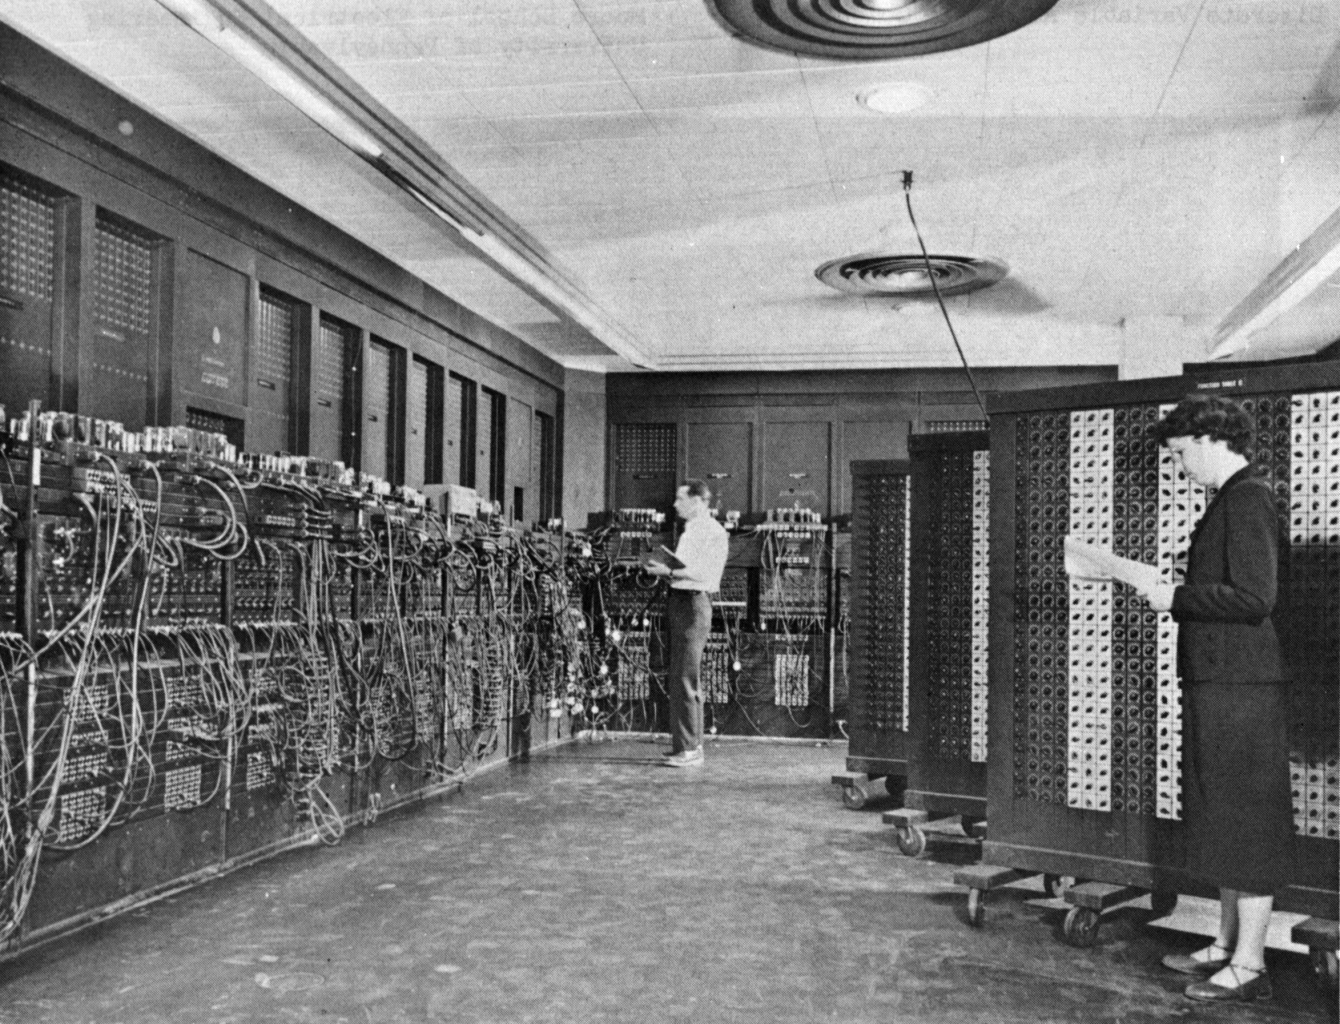
\includegraphics [width=.8\textwidth] {\inc/eniac}
	\\
	\creditphoto {U.S. Army} {domaine public}
    \end {center}

\end {frame}

\begin {frame} {Historique -- Les premiers ordinateurs}

    Sur ces ordinateurs~:

    \begin {itemize}
	\item programmer : câbler des connexions entre les unités

	\item résultats : à consulter sur des indicateurs lumineux

    \end {itemize}

    L'ordinateur~:
    \begin {itemize}
	\item est très onéreux (généralement un seul exemplaire)
	\item est très difficile à programmer (6 programmeuses à l'origine
	    sur l'ENIAC, la programmation dure plusieurs semaines)
	\item se programme par câblage physique
	\item n'exécute qu'un seul programme à la fois
	\item n'a pas ou peu de périphériques
    \end {itemize}

    \implique pas de système d'exploitation

\end {frame}


\begin {frame} {Historique -- Démarrage aux clefs}

    Étape suivante~:

    \begin {center}
	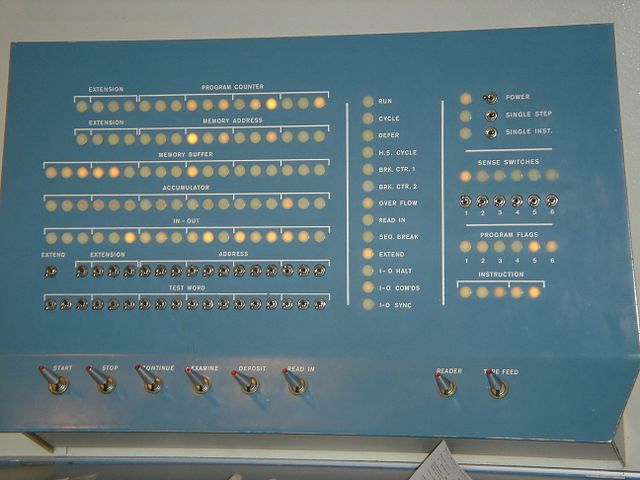
\includegraphics [width=.5\textwidth] {\inc/pdp1}
	\\
	\creditphoto {"PDP-1 control board" by fjarlq / Matt - http://www.flickr.com/photos/fjarlq/147938903/} {\ccby}
    \end {center}

    \begin {itemize}
	\item panneau de commande de l'ordinateur
	\item saisie du programme en mémoire avec des interrupteurs
	\item lancement du programme avec un interrupteur
	\item lecture du résultat avec les indicateurs lumineux
    \end {itemize}
    \implique pas de système d'exploitation

\end {frame}


\begin {frame} {Historique -- Carte perforée}

    La carte perforée (début des années 1950)

    \begin {minipage} [c] {.40\textwidth}
    \begin {center}
	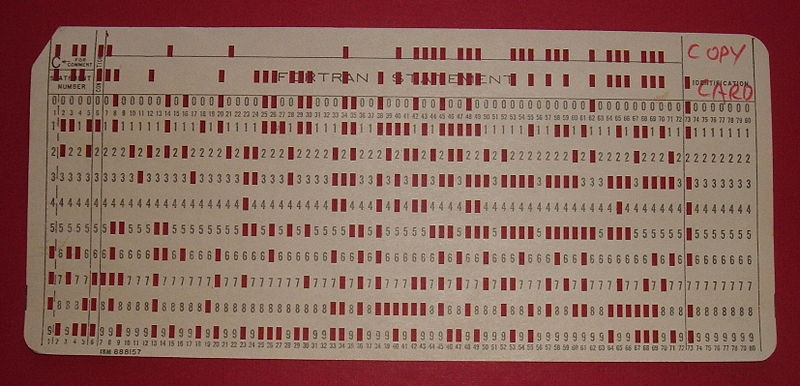
\includegraphics [width=\textwidth] {\inc/carte-perfo}
	\\
	\creditphoto {Arnold Reinhold} {\ccbysa}
    \end {center}
    \end {minipage}
    \hfill
    \begin {minipage} [c] {.58\textwidth}
    \begin {center}
	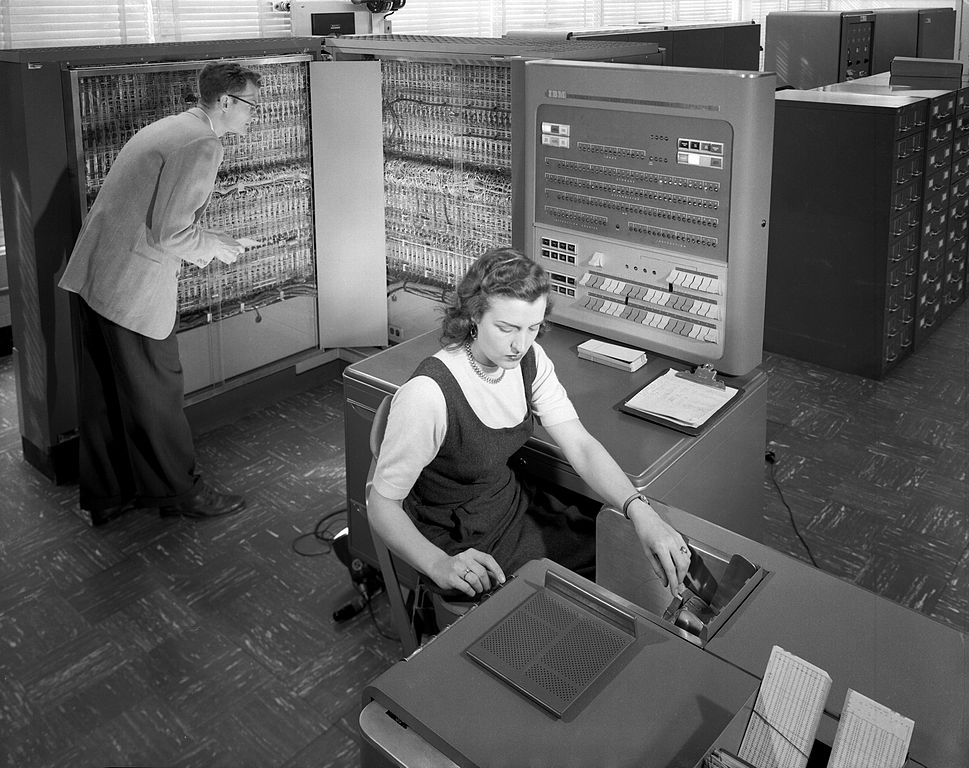
\includegraphics [width=\textwidth] {\inc/ibm704}
	\\
	\creditphoto {NASA (IBM 704)} {domaine public}
    \end {center}
    \end {minipage}

    \begin {itemize}
	\item périphérique d'entrée des programmes (et des données)
	\item programme en mémoire (morte) pour démarrer le lecteur,
	    stocker le programme en mémoire, et lancer son exécution
    \end {itemize}

\end {frame}

\begin {frame} {Historique -- Moniteur}

    Carte perforée \implique entrée automatisée des programmes

    \vspace* {3mm}

    Cependant :

    \begin {itemize}
	\item intervention d'un opérateur humain pour :
	    \begin {itemize}
		\item placer le bac de cartes dans le lecteur
		\item lancer la lecture
		\item attendre la fin du programme
		\item récupérer les résultats (sur l'imprimante)
	    \end {itemize}

	\item l'ordinateur est très onéreux : toute minute de calcul
	    perdue coûte cher !

    \end {itemize}

    D'où : programmes « \textbf {moniteurs} » résidant en mémoire

    \begin {itemize}
	\item toujours un seul programme à la fois
	\item automatisation du passage des différents programmes
	\item traitement par « lot » (de cartes) \implique
	    \textbf {batch processing}
	\item accès facilité aux périphériques
	\item premiers embryons de systèmes d'exploitation
    \end {itemize}

\end {frame}

\begin {frame} {Historique -- Spooling}
    Ordinateur onéreux \implique mieux le rentabiliser ?

    \begin {itemize}
	\item certains périphériques (lecteur de cartes perforées,
	    imprimante) sont lents

	    \includegraphics [width=.9\textwidth] {\inc/spool1}


	\item peut-on lancer un calcul pendant que les périphériques
	    lents travaillent ?

	    \includegraphics [width=.9\textwidth] {\inc/spool2}

    \end {itemize}

\end {frame}

\begin {frame} {Historique -- Spooling}
    Exemple~: IBM 7094 (1963)

    \begin {center}
	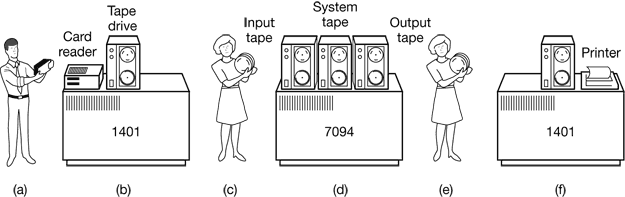
\includegraphics [width=.8\textwidth] {\inc/spool-tanenb}
	\\
	\credit {Extrait de Tanenbaum, A.S., Woodhull A.S.,
		« Operating Systems, Design and Implementation »,
		3rd ed, Pearson}
    \end {center}

    \begin {itemize}
	\item IBM 7094 : très onéreux
	\item IBM 1401 : peu coûteux (pour l'époque) \\
	    \implique dédié aux
	    transferts entre périphériques lents et bandes magnétiques
	    (rapides)
	\item transfert manuel des bandes \\
	    \implique évolution vers une connexion directe \\
	    \implique évolution vers des disques durs

    \end {itemize}
\end {frame}

\begin {frame} {Historique -- Spooling}
    En résumé :

    \begin {itemize}
	\item évolution vers des « périphériques » plus
	    « intelligents »
	\item fonctionnent en parallèle avec le processeur
	    central

    \end {itemize}

    \vspace* {3mm}

    \implique il faut maintenant tirer parti de ce parallélisme

    \begin {itemize}
	\item le moniteur doit gérer les ressources matérielles lentes
	    pour en exploiter le parallélisme
    \end {itemize}
\end {frame}

\begin {frame} {Historique -- Multi-programmation}
    Et lorsque le programme attend le résultat d'une entrée/sortie ?

    \begin {itemize}
	\item « démocratisation » des périphériques
	\item ex: stockage ou récupération d'une donnée temporaire
	    sur un périphérique (bande magnétique, disque dur, etc.)

	\item temps mort pour le processeur \\
	    \implique utiliser ce temps mort pour un autre programme

    \end {itemize}

    \vspace* {3mm}

    Introduction de la multi-programmation \implique \textbf {superviseur}
\end {frame}

\begin {frame} {Historique -- Multi-programmation}

    Le superviseur charge plusieurs programmes en mémoire~:
    \begin {itemize}

	\item lorsque le programme en cours demande une E/S, le
	    superviseur démarre le programme suivant
	\item lorsque le contrôleur d’E/S signale la fin de l’E/S,
	    le premier programme reprend son exécution
    \end {itemize}

    \vspace* {3mm}

    Exemple~: Atlas Supervisor de l'U. de Manchester (1962)
\end {frame}

\begin {frame} {Historique -- Multi-programmation}
    Questions posées par la multiprogrammation~:

    \begin {itemize}
	\item comment protéger les programmes les uns des autres ?
	    \\
	    \implique accès interdit aux variables d'un autre programme

	    \implique \textbf {unité de gestion mémoire} (composant matériel)

	\item comment le superviseur reprend le contrôle
	    lorsque le contrôleur d'E/S a terminé ?

	    \implique \textbf {mécanisme d'interruptions}
    \end {itemize}

\end {frame}

\begin {frame} {Historique -- Télétype}
    \begin {minipage} [c] {.40\textwidth}
    \begin {center}
	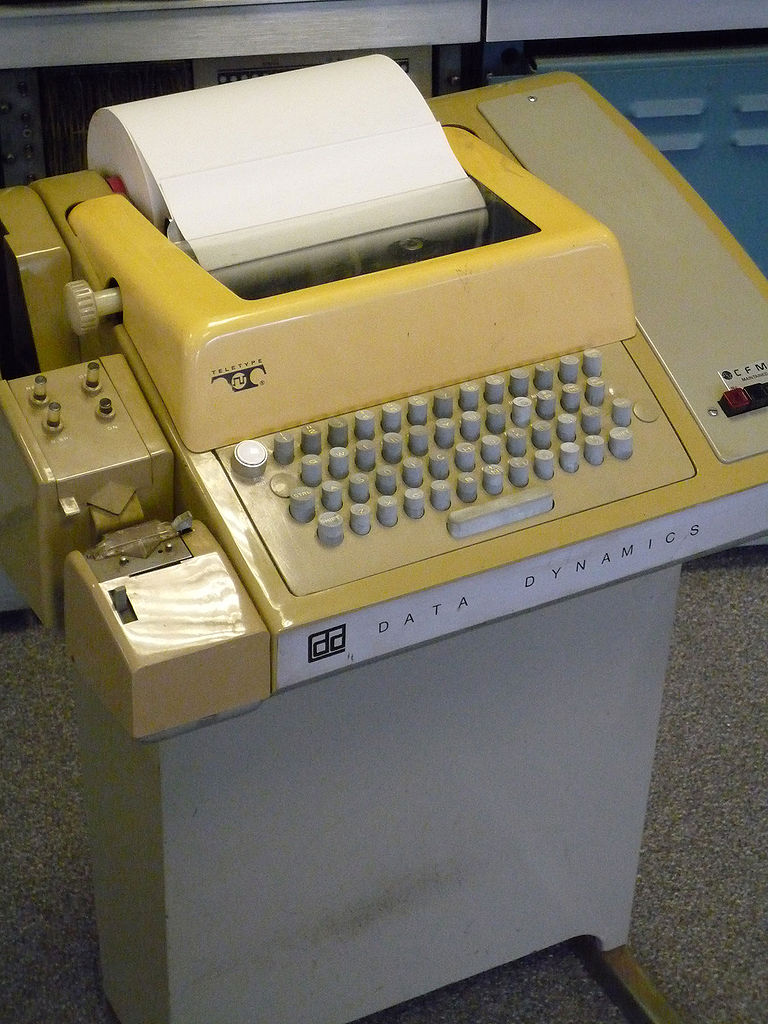
\includegraphics [width=\textwidth] {\inc/tty}
	\\
	\creditphoto {AlisonW} {\ccbysa}
    \end {center}
    \end {minipage}
    \hfill
    \begin {minipage} [c] {.58\textwidth}
	Ceci est une révolution !
	\begin {itemize}
	    \item changement fondamental dans l'interaction
		avec l'ordinateur
	    \item plus besoin d'attendre le passage du bac de
		cartes perforées sur l'ordinateur
	    \item commandes tapées au clavier \\
		\implique langage de commandes
	    \item résultat directement imprimé
	\end {itemize}
    \end {minipage}

\end {frame}

\begin {frame} {Historique -- Télétype}

    \begin {itemize}
	\item c'est un périphérique comme un autre...

	\item ... mais l'interaction modifie le besoin

	\item le superviseur lance des actions suite à des
	    commandes tapées à la console

	\item usage « interactif » $\neq$ usage « batch »

    \end {itemize}

\end {frame}

\begin {frame} {Historique -- Temps partagé}
    Connecter plusieurs terminaux à un même ordinateur :

    \begin {itemize}
	\item accueillir plusieurs utilisateurs
	\item mieux rentabiliser le coût d'un ordinateur
	\item connexion via une liaison série directe, ou via un modem
	\item donner à chacun l'impression d'avoir « son » ordinateur
	\item systèmes à temps partagé
    \end {itemize}

    Exemples~:
    \begin {itemize}
	\item CTSS (Compatible Time-Sharing System) : MIT (1961)
	    \\
	    IBM 7094 modifié par IBM, 32 utilisateurs maximum
	\item STSS (Stanford Time-Sharing System) : Stanford (1963)
	    \\
	    DEC PDP-1, 12 terminaux
    \end {itemize}
\end {frame}

\begin {frame} {Historique -- Temps partagé}
    Allouer le processeur pendant des petites portions de temps à
    chaque utilisateur~:

    \begin {itemize}
	\item quantum : durée fixée par le système (ex: 20 ms)
	\item pour un être humain, les programmes semblent tourner
	    en parallèle
    \end {itemize}


    \begin {center}
	\includegraphics [width=.9\textwidth] {\inc/quantum}
    \end {center}

\end {frame}

\begin {frame} {Historique -- Temps partagé}
    Questions posées par le temps partagé~:

    \begin {itemize}
	\item comment reprendre le contrôle à la fin de quantum ?
	    \\
	    \implique mécanisme d'\textbf {horloge} avec interruption

	\item comment gérer plusieurs utilisateurs ?
	    \\
	    \implique identité : validation et autorisations \\
	    \implique mécanismes logiciels

	\item comment éviter qu'un utilisateur outrepasse ses droits ?
	    \\
	    \implique \textbf {modes d'exécution} privilégié et non
		privilégié \\
	    \implique quelques instructions interdites en mode non
		privilégié

	    \vspace* {1mm}

	    Exemple~:
	    \begin {itemize}
		\item accès au disque : réservé au mode
		    privilégié
		\item programmes utilisateurs : exécutés
		    en mode non privilégié
		    \\
		    \implique passage par le système pour
		    accéder aux fichiers
	    \end {itemize}

    \end {itemize}

\end {frame}

\begin {frame} {Historique -- Appel système}
    Lorsqu'un programme souhaite effectuer (par exemple) un accès
    disque, il fait un \textbf {appel système} :

    \begin {itemize}
	\item instruction spéciale (TRAP, SVC, INT, etc. suivant le
	    processeur)

	\item provoque (entre autres) :
	    \begin {itemize}
		\item basculement en mode privilégié
		\item déroutement du programme vers une adresse spécifique
	    \end {itemize}

	\item adresse spécifique = système d'exploitation
	\item \textbf {vérification} des paramètres, des droits, etc.
	    \\
	    \implique pour éviter qu'un utilisateur outrepasse ses droits
	\item réalisation de l'action demandée par l'appel système

    \end {itemize}

\end {frame}

\begin {frame} {Historique -- Temps partagé}

    Début des années 1970 : terminaux à écran cathodique

    \begin {center}
	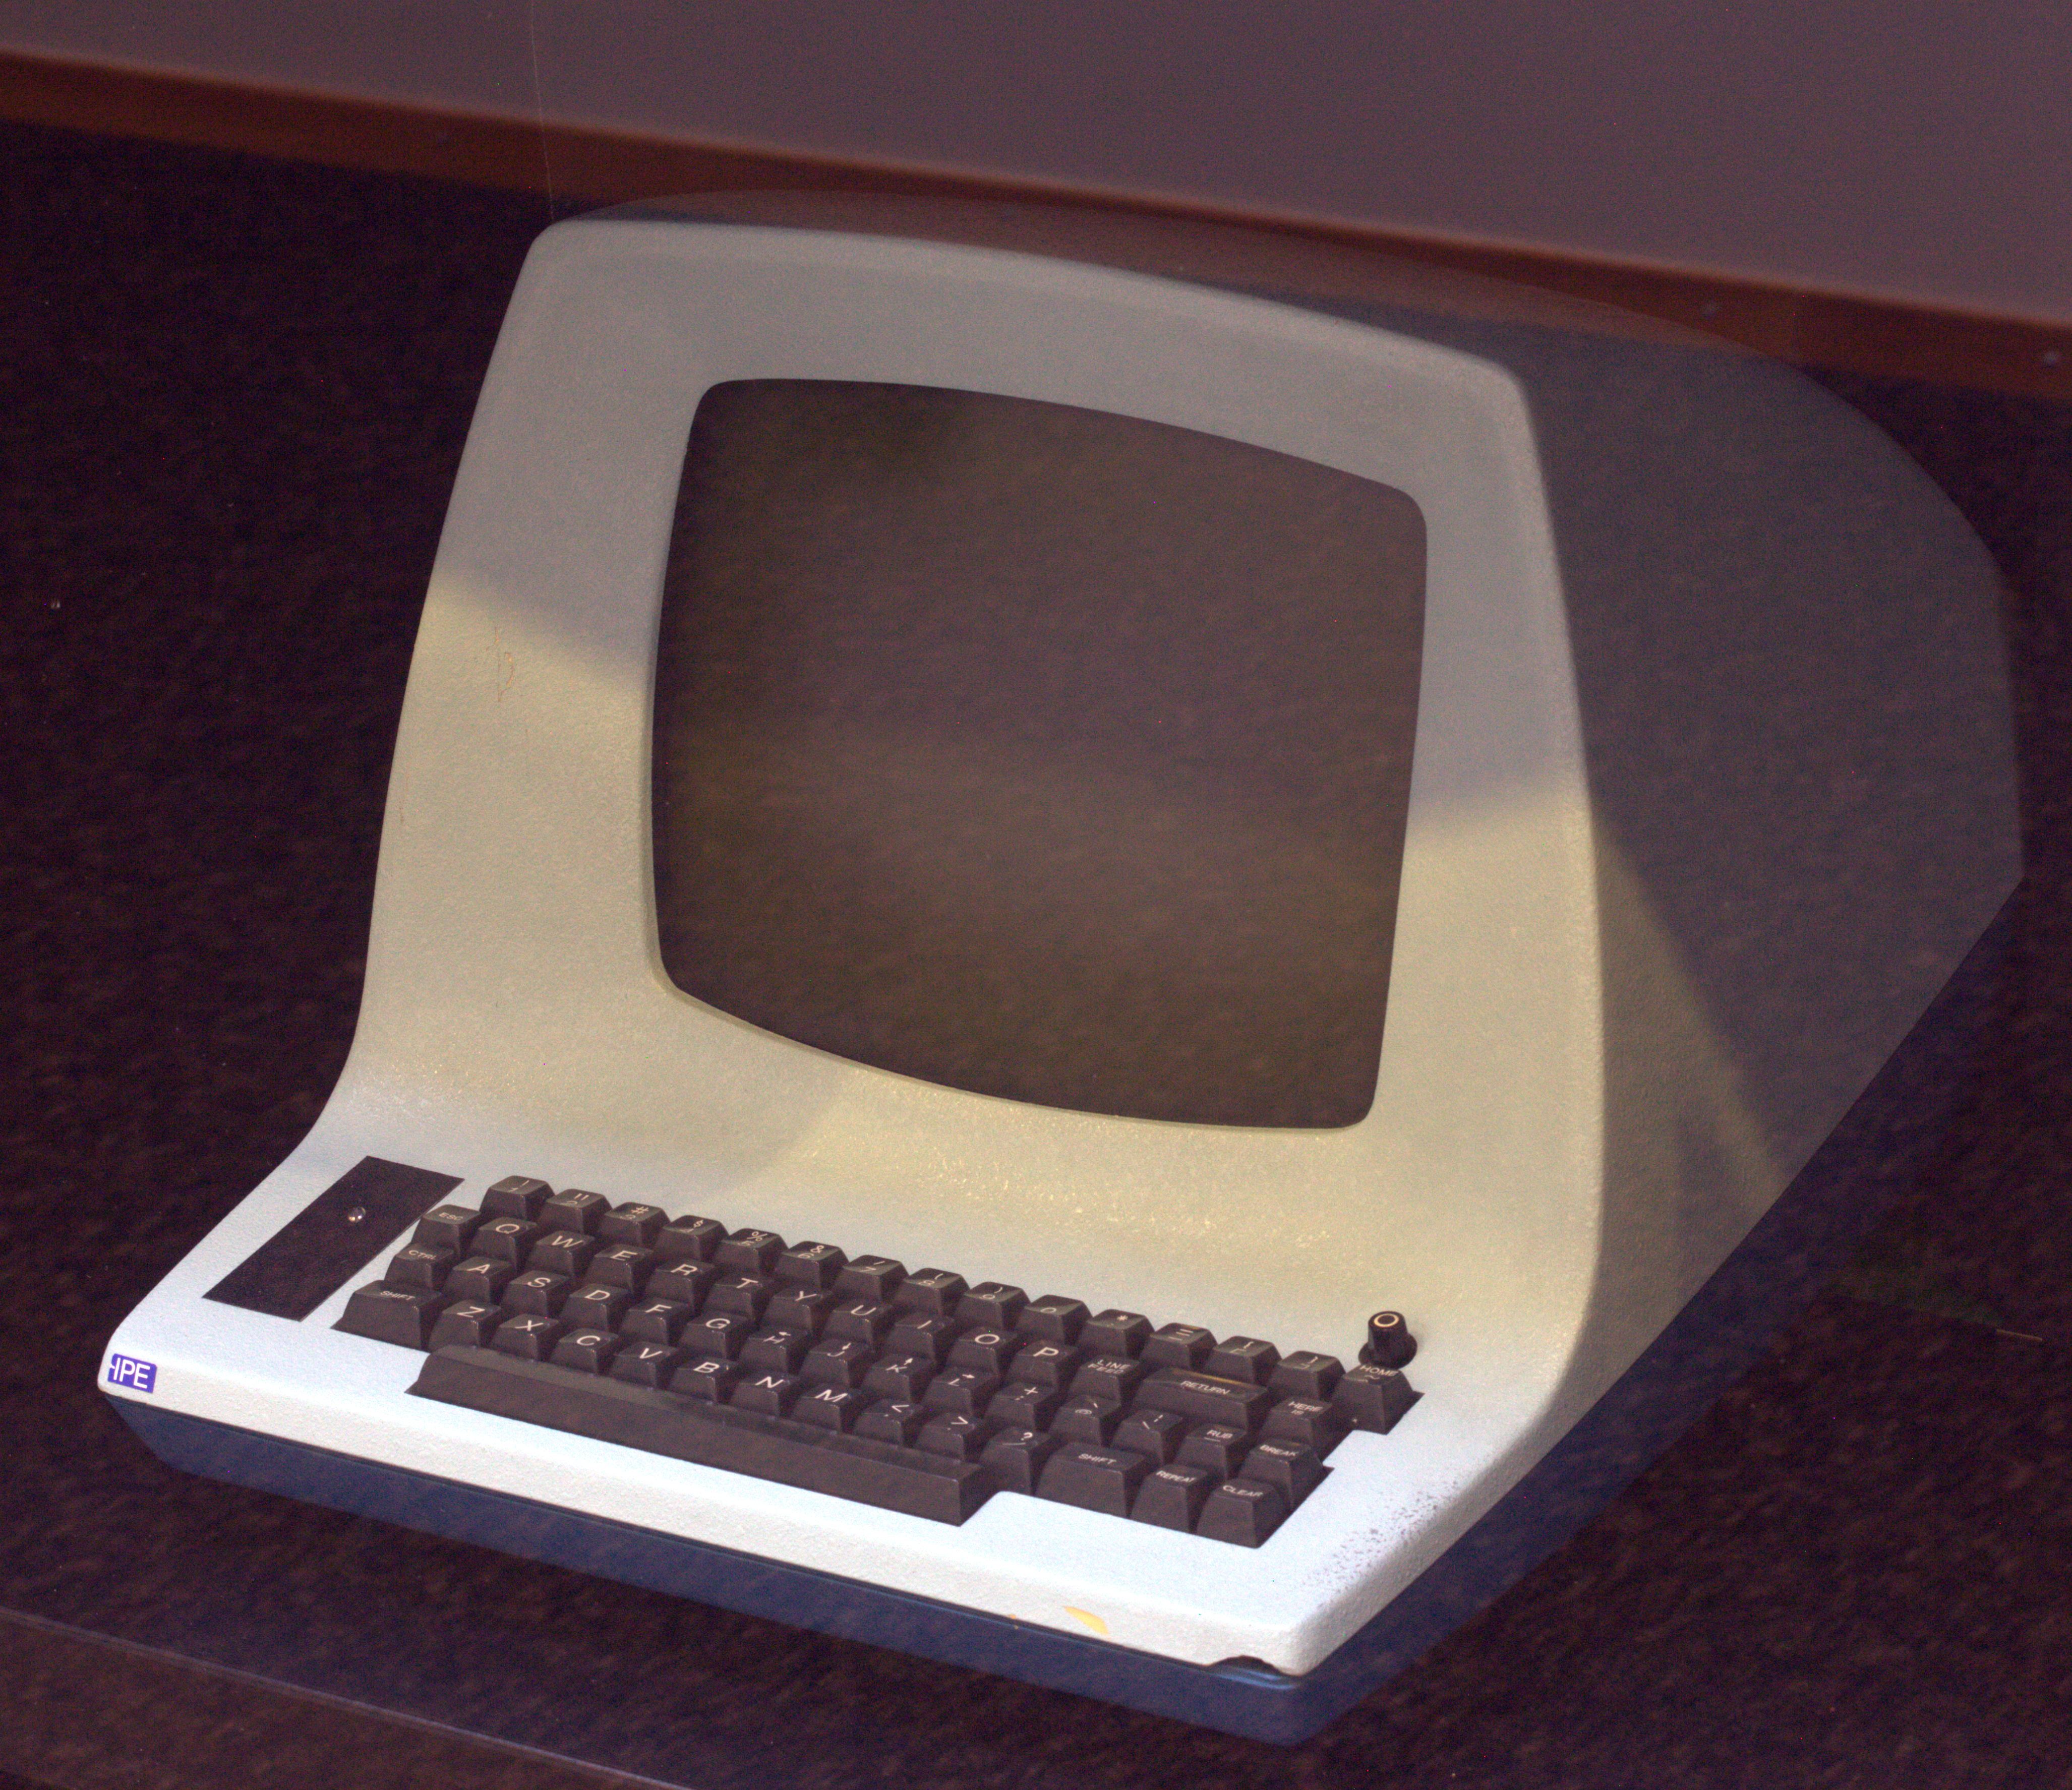
\includegraphics [width=.4\textwidth] {\inc/term-adm3a}
	\\
	\creditphoto {"Lear Siegler ADM-3A-IMG 1508" by Photograph by
	Rama} {\ccbysa}
    \end {center}

    \vspace* {3mm}

    Âge d'or des « mainframes »

    \implique stabilisation des systèmes d'exploitation autour des
    concepts vus précédemment

\end {frame}

\begin {frame} {Bilan}
    Fonctionnalités offertes par un système d'exploitation

    \begin {itemize}
	\item rentabiliser l'usage de l'ordinateur
	    \\
	    \implique utiliser tous les temps morts
	\item partager un ordinateur entre plusieurs utilisateurs
	    \\
	    \implique partager équitablement les ressources matérielles

	\item faciliter l'accès aux périphériques
	    \\
	    \implique offrir une interface avec le matériel
	    \\
	    \implique pour tirer parti du parallélisme des périphériques

	\item permettre à des utilisateurs d'éditer, développer,
	    lancer des programmes
    \end {itemize}

    ... le tout en offrant les garanties de sécurité nécessaires
\end {frame}

%%%%%%%%%%%%%%%%%%%%%%%%%%%%%%%%%%%%%%%%%%%%%%%%%%%%%%%%%%%%%%%%%%%%%%%%%%%%%%
% Le noyau
%%%%%%%%%%%%%%%%%%%%%%%%%%%%%%%%%%%%%%%%%%%%%%%%%%%%%%%%%%%%%%%%%%%%%%%%%%%%%%

\titreB {Le noyau}

\begin {frame} {Continuons l'historique}

    Systèmes d'exploitation marquants~:

    \begin {itemize}
	\item Burroughs MCP (1961)
	    \begin {itemize}
		\item conçu pour l'ordinateur Burroughs B5000
		\item premier SE programmé en \textbf {langage de
		    haut niveau}
		\item beaucoup d'éléments innovants (multiprocesseurs,
		    mémoire virtuelle)
	    \end {itemize}
	\item IBM OS/360 (1964)
	    \begin {itemize}
		\item SE « universel » pour les ordinateurs IBM System/360
		\item énorme (des dizaines de millions de lignes d'assembleur)
		\item \textbf {complexe}, beaucoup de retards
		\item F. Brooks « The Mythical Man-Month »
	    \end {itemize}
	\item CTSS (\textbf {MIT}, 1961)
	    \begin {itemize}
		\item premier système multi-utilisateurs
		\item IBM 7094 modifié (2 exemplaires)
	    \end {itemize}
    \end {itemize}

\end {frame}

\begin {frame} {Multics}

    \begin {itemize}
	\item Multics (MULtiplexed Information and Computing Service)
	    \begin {center}
		\fD
		\begin {tabular} {|l|l|} \hline
		    \rca 1963 & spécification (MIT) \\
		    \rcb 1964 & démarrage du projet \\
		    \rca 1964 & General Electric + Bell Labs rejoignent le MIT \\
		    \rcb 1968 & première version « self-hosting » \\
		    \rca 1969 & \textbf {Bell Labs} se retirent du projet \\
		    \rcb 1973 & annonce commerciale \\
		    \rca 1985 & fin du développement \\
		    \rcb 2000 & fermeture du dernier site (Min Défense Canada) \\
		    \hline
		\end {tabular}
	    \end {center}

	    \begin {itemize}
		\item Système très ambitieux
		\begin {itemize}
		    \item écrit en langage de haut niveau (PL/1)
		    \item accès uniforme à la mémoire et aux fichiers
		    \item système de fichiers hiérarchique
		    \item édition de liens dynamique
		    \item reconfiguration matérielle dynamique
		    \item processus « démons »
		    \item sécurité (certification B2 en 1985)
		\end {itemize}
		\item 84 sites au total (dont 31 universités/centres français)
	    \end {itemize}
    \end {itemize}

\end {frame}

\begin {frame} {Unix}

    \begin {itemize}
	\item Unix
	    \begin {center}
		\fD
		\begin {tabular} {|l|l|} \hline
		    \rca 1969 & Bell Labs se retirent du projet Multics \\
		    \rca      & récupération d'un PDP-7, écriture en assembleur \\
		    \rcb 1971 & achat PDP-11/20 en échange d'un formateur de texte \\
		    \rca 1972 & création du langage C et réécriture d'Unix en C \\
		    \rcb 1973 & premières diffusions \\
		    \rca 1979 & Unix v7 (environ 10 000 lignes de C et un peu
			d'assembleur) \\
		    \rcb 1980 & distribution 4BSD \\
		    \rca 1992 & procès AT\&T vs BSDi vs Berkeley (fin en 1994) \\
		    \hline
		\end {tabular}
	    \end {center}

	    \begin {itemize}
		\item Beaucoup d'idées novatrices
		    \begin {itemize}
			\item simple
			\item écrit en langage C
			\item séparation nette \textbf {noyau} / utilitaires
			    (ou applications)
			\item tout est fichier
			\item pas de structure interne des fichiers
			\item interface utilisateur simple (minimaliste)
			\item philosophie Unix (kiss : « keep it simple, stupid »)
			\item portable
		    \end {itemize}
	    \end {itemize}
	    
    \end {itemize}

\end {frame}

\begin {frame} {Le noyau}
    Philosophie Unix \implique approche minimaliste,
    à l'opposé des systèmes d'exploitation précédents

    \vspace* {3mm}

    Le noyau a deux objectifs fondamentaux~:
    \begin {itemize}
	\item \textbf {partager équitablement les ressources}
	\item \textbf {garantir la sécurité des données}
    \end {itemize}

\end {frame}

\begin {frame} {Le noyau}
    Partager équitablement les ressources~:

    \begin {itemize}
	\item mémoire vive
	\item temps processeur
	\item carte réseau
	\item espace disque
	\item accès aux disques
	\item etc.
    \end {itemize}
\end {frame}

\begin {frame} {Le noyau}
    Garantir la sécurité des données

    \begin {itemize}
	\item un processus ne doit pas accéder aux données d'un autre
	    processus (sauf si autorisé)

	\item un utilisateur ne doit pas accéder à un fichier non autorisé

	\item un utilisateur ne doit pas terminer un processus d'un
	    autre utilisateur

	\item etc.

    \end {itemize}
\end {frame}

\begin {frame} {Le noyau}

    Pour atteindre les deux objectifs fondamentaux :

    \begin {itemize}
	\item le \textbf {noyau} s'exécute en \textbf {mode privilégié}
	    \\
	    \implique il a accès à toutes les ressources matérielles

	\item les programmes (applications) s'exécutent, dans le
	    contexte de \textbf {processus}, en \textbf {mode non
	    privilégié}
	    \\
	    \implique appels au noyau pour exécuter certaines opérations

    \end {itemize}

    \vspace* {3mm}

    Les appels au noyau sont les \textbf {primitives systèmes}

    \begin {itemize}
	\item Interface de programmation du noyau
	    \\
	    \textit {Application Programming Interface} (API)
	\item Forme : appels de fonction en C
	\item Exemple :
	    \\
	    \code {int open (const char *path, int flag, mode\_t mode)}
    \end {itemize}


\end {frame}

\begin {frame} {Le noyau}
    \begin {center}
	\includegraphics [width=.7\textwidth] {\inc/noyau}
    \end {center}
\end {frame}

\begin {frame} {Le noyau}
    Définition :

    \begin {quote}
	Le noyau est constitué de l'ensemble minimum des primitives
	systèmes nécessaires pour atteindre les deux objectifs
	fondamentaux

    \end {quote}

\end {frame}

\begin {frame} {Le noyau}
    \begin {itemize}
	\item Démarrage de l'ordinateur : noyau installé
	    en mémoire \\
	    \implique il y restera jusqu'à la fin (redémarrage,
	    arrêt, ou crash)

	\item Le noyau s'exécute en mode privilégié

	    \begin {itemize}
		\item code sensible
		\item difficile à développer, à mettre au point
		\item plus il est petit, mieux c'est
		\item tout ce qui peut être mis ailleurs doit l'être
		    \\
		    \vspace* {0.8mm}
		    Exemple :
		    \begin {itemize}
			\item pour le noyau, un utilisateur = un nombre
			    entier
			\item \code {ls -l} affiche des noms de login
			\item \implique la conversion
			    « entier $\leftrightarrow$ nom » est
			    effectuée par \code {ls}

		    \end {itemize}
	    \end {itemize}

	\item Mise en évidence du concept de noyau \\
	    \implique apport majeur d'Unix

    \end {itemize}

\end {frame}

\begin {frame} {Le noyau}
    Quelles fonctions doivent être des primitives systèmes ?

    \begin {itemize}
	\item un processus ne doit pas avoir le droit d'accéder
	    directement au disque (violation du deuxième objectif)
	    \\
	    \implique il faut que le noyau présente une abstraction avec
	    des droits : système de fichiers, propriétaire,
	    droits d'accès \\
	    \implique accès au disque par l'intermédiaire de cette
	    abstraction
	    \\
	    \implique \code {open} est une primitive système

	\item lire l'heure courante \implique accès à un périphérique
	    \\
	    \implique \code {time} est une primitive système

    \end {itemize}
\end {frame}

\begin {frame} {Le noyau}
    Quelles fonctions doivent être des primitives systèmes ?

    \begin {itemize}
	\item \code {strlen} calcule un nombre d'octets en lisant
	    dans la mémoire du processus courant (donc autorisé)
	    \\
	    \implique \code {strlen} n'est donc pas une primitive système

	    \vspace* {1mm}

	    Comme elle est utile, on la met\footnote {Ou plutôt son code
	    compilé.} dans une \textbf {bibliothèque} une fois pour
	    toutes, pour éviter d'avoir à la reprogrammer à chaque fois

	\item \code {getlogin} renvoie le nom de login de l'utilisateur
	    \\
	    \implique cette fonction récupère le numéro de
	    l'utilisateur avec une primitive système, puis convertit ce
	    numéro en nom en parcourant le fichier \code {/etc/passwd}
	    (ou en utilisant une base externe LDAP dans le cas de turing)
	    \\
	    \implique \code {getlogin} n'est pas une primitive système

    \end {itemize}
\end {frame}

\begin {frame} {Interface utilisateur}
    \begin {center}
    \fD
    \begin {tabular} {|l|l|l|} \hline
	\rca Date & \multicolumn {1} {c|} {Stations de travail}
		& \multicolumn {1} {c|} {Ordinateurs personnels}
	    \\ \hline
	\rcb 1968 & \multicolumn {2} {l|} {Prototype de souris par
		Douglas Englebart (Stanfort Research Institute)} \\
	\rca 1973 & Alto (Xerox) & \\
	\rcb 1981 & Display Manager (Apollo Computer) & \\
	\rca 1983 & W Window System (Stanford) & Lisa (Apple) \\
	\rcb 1984 & X Window System (MIT) & \\
	\rca 1985 & HP Windows (HP),	& Amiga Workbench (Commodore), \\
	\rca      & Sunview (Sun)	& Windows (Microsoft), etc \\
	\hline
    \end {tabular}
    \end {center}

    La gestion d'une interface utilisateur « graphique » n'est pas
    du ressort du noyau :
    \begin {itemize}
	\item Souris, écran graphique, écran tactile (tablette, etc.) \\
	    \implique périphériques gérés par le noyau
	\item Système de fenêtrage \\
	    \implique applications
    \end {itemize}
\end {frame}

\begin {frame} {Qu'est-ce qu'un système d'exploitation ?}
    Retour sur notre interrogation du début :
    \begin {itemize}
	\item Unix (l'original, puis les *BSD) : noyau + applications
	\item Linux est un noyau
	    \begin {itemize}
		\item des organisations (bénévoles ou commerciales) ont
		    réuni des applications, les ont compilées et ont
		    diffusé, avec le noyau, des \textbf {distributions}
		    prêtes à l'emploi

	    \end {itemize}
	\item Windows : noyau + applications
	\item Android, iOS : noyau (avec support de périphériques tactiles,
	    audio, GSM, GPS, etc.) + applications
	\item box Internet, montre connectée, voiture, etc. : noyau
	    +  applications spécifiques
	\item etc.
    \end {itemize}
\end {frame}

\begin {frame} {Quelques systèmes atypiques}
    \begin {itemize}
	\item systèmes temps réel
	\item systèmes contraints (ex: Internet des Objets)
    \end {itemize}
\end {frame}

\begin {frame} {Bilan}
    \begin {itemize}
	\item Depuis Unix : distinction entre noyau et reste du système
	    d'exploitation

	\item Objet de cette UE : comprendre le fonctionnement d'un noyau
	    de système d'exploitation

    \end {itemize}

\end {frame}

%%%%%%%%%%%%%%%%%%%%%%%%%%%%%%%%%%%%%%%%%%%%%%%%%%%%%%%%%%%%%%%%%%%%%%%%%%%%%%
% POSIX
%%%%%%%%%%%%%%%%%%%%%%%%%%%%%%%%%%%%%%%%%%%%%%%%%%%%%%%%%%%%%%%%%%%%%%%%%%%%%%

\titreB {POSIX}

\begin {frame} {Interface des primitives systèmes}
    Primitives systèmes = ensemble de fonctions (appelables en C)
    pour accéder aux services offerts par le noyau

    \begin {itemize}
	\item À l'origine (Unix v6, 1975) : 43 primitives
	\item Évolutions ultérieures (années 1980) :
	    \begin {itemize}
		\item Bell Labs, AT\&T
		\item U. de Berkeley
		\item Essor commercial
	    \end {itemize}
	\item Résultat
	    \begin {itemize}
		\item de nombreuses divergences \implique incompatibilités
		\item les programmes ne sont plus portables
		\item les utilisateurs ne sont pas contents
	    \end {itemize}
	\item Il faut normaliser l'existant \implique POSIX
    \end {itemize}

\end {frame}

\begin {frame} {POSIX}

    Comité POSIX de l’IEEE
    \begin {itemize}
	\item IEEE = Institute of Electrical and Electronics Engineers
	    \\
	    (association américaine, rédige des textes normatifs)
	\item POSIX = Portable Operating System Interface
	\item Norme IEEE : IEEE Std 1003.*
	\item Norme internationale : ISO/IEC 9945
	\item Première version : 1988
	\item Version actuelle : 2013
    \end {itemize}

    \vspace* {3mm}

    Impact majeur \implique aucun système d'exploitation ne peut
    se permettre de ne pas être compatible POSIX
\end {frame}

\begin {frame} {POSIX}

    POSIX normalise beaucoup de choses :

    \begin {itemize}
	\item des primitives systèmes et des fonctions de bibliothèque
	\item des commandes (\code {sh}, \code {ls}, \code {tr}, etc.)
	\item des extensions (temps réel, threads, sémaphores, etc.)
    \end {itemize}

    \vspace* {3mm}

    POSIX ne normalise pas tout :
    \begin {itemize}
	\item une implémentation peut avoir ses propres extensions \\
	    \implique non normalisées \implique non portables
	\item Exemple avec \code {ls} :
	    \begin {itemize}
		\item POSIX 2013 : 23 options (c'est beaucoup...) \\
		\item GNU (Linux) : 58 options (c'est trop !) \\
	    \end {itemize}
	\item programmer portable \implique respecter POSIX
	\item utiliser la notice fournie en cours

    \end {itemize}

\end {frame}

\begin {frame} {POSIX}

    POSIX ne fait pas de distinction entre primitive système et fonction
    de bibliothèque :

    \begin {itemize}
	\item laisser de la liberté pour les implémentations
	\item distinction parfois mince
	    \begin {itemize}
		\item Exemple : 6 fonctions pour exécuter un programme
		    (\code {execv}, \code {execl}, \code {execvp},
		    \code {execlp}, \code {execve} et \code {execle}),
		    une seule est une primitive, les 5 autres sont des
		    fonctions de bibliothèque
	    \end {itemize}
    \end {itemize}
\end {frame}

\begin {frame} {POSIX}
    Principes généraux

    \begin {itemize}
	\item Types POSIX
	\item Constantes
	\item Gestion des erreurs
	\item Paramètres de type « pointeur »
    \end {itemize}
\end {frame}

\begin {frame} {POSIX -- Types}
    \begin {itemize}
	\item Le noyau Unix manipulait des objets grâce à des entiers

	    \vspace* {1mm}
	    Problème : portabilité (16/32/64 bits ? implémentations ?)

	\item POSIX a introduit de nouveaux types (avec \code {typedef})
	    \\
	    \implique masquer le détail d'implémentation \\
	    \implique portabilité des programmes

	    \vspace* {1mm}
	    Quelques exemples :

	    \begin {center}
	    \fC
	    \begin {tabular} {|l|l|} \hline
		\rca \code {uid\_t} & numéro d'utilisateur \\
		\rcb \code {gid\_t} & numéro de groupe \\
		\rca \code {pid\_t} & numéro de processus \\
		\rcb \code {mode\_t} & permissions \\
		\rca \code {time\_t} & heure courante \\
		\rcb \code {size\_t} & taille, résultat de sizeof (définie par ISO C) \\
		\hline
	    \end {tabular}
	    \end {center}

	    Définitions des types : fichiers d'inclusion
    \end {itemize}

\end {frame}

\begin {frame} {POSIX -- Constantes}
    \begin {itemize}
	\item Certaines primitives nécessitent de spécifier une opération

	\item Exemple~:
	    \begin {center}
		\fC
		\begin {tabular} {|l|l|} \hline
		    \rca \code {r = access ("toto", 0)}
			& le fichier existe-t'il ? \\
		    \rcb \code {r = access ("toto", 1)}
		    	& puis-je exécuter le fichier ? \\
		    \rca \code {r = access ("toto", 2)}
		    	& puis-je modifier le fichier ? \\
		    \rcb \code {r = access ("toto", 4)}
			& puis-je lire le fichier ? \\
		    \hline
		\end {tabular}
	    \end {center}

	    \vspace* {3mm}

	\item Il faut se rappeler des valeurs et de leur signification
    \end {itemize}

\end {frame}

\begin {frame} {POSIX -- Constantes}
    \begin {itemize}

	\item Définition de constantes (dans les fichiers d'inclusion)

	    Fichier \code {unistd.h} :
	    \lstinputlisting [basicstyle=\fD\lstmonstyle] {\inc/unistd.h}

	\item L'exemple précédent devient :
	    \begin {center}
		\fC
		\begin {tabular} {|l|l|} \hline
		    \rca \code {r = access ("toto", F\_OK)}
			& le fichier existe-t'il ? \\
		    \rcb \code {r = access ("toto", X\_OK)}
		    	& puis-je exécuter le fichier ? \\
		    \rca \code {r = access ("toto", W\_OK)}
		    	& puis-je modifier le fichier ? \\
		    \rcb \code {r = access ("toto", R\_OK)}
			& puis-je lire le fichier ? \\
		    \hline
		\end {tabular}
	    \end {center}
	    \vspace* {2mm}

	\item Utiliser les constantes rend les programmes plus lisibles

	\item Parfois, les constantes sont moins pratiques (permissions)
	    ou peu répandues

    \end {itemize}

\end {frame}

\begin {frame} {POSIX -- Constantes}
    Certaines constantes ne sont pas constantes...

    \begin {itemize}
	\item arguments sémantiques des primitives : fichiers d'inclusion
	    \begin {center}
		\fE
		Exemples~:
		\begin {tabular} {|l|l|l|} \hline
		    \rca \code {R\_OK}
			& test en lecture pour \code {access}
			& \code {unicode.h}
			\\
		    \rcb \code {O\_WRONLY}
			& ouverture en écriture pour \code {open}
			& \code {fcntl.h}
			\\
		    \rca \code {S\_IFDIR}
			& type de fichier « répertoire »
			& \code {sys/stat.h}
			\\
		    \rcb ... & &
			\\
			\hline
		\end {tabular}
	    \end {center}

	\item limites arbitraires : \code {limits.h}
	    \begin {center}
		\fE
		Exemples~:
		\begin {tabular} {|l|l|} \hline
		    \rca \code {PATH\_MAX}
			& taille maximum des chemins
			\\
		    \rca \code {LOGIN\_NAME\_MAX}
			& nombre maximum d'ouvertures de fichier
			\\
		    \rcb \code {CHILD\_MAX}
			& nombre maximum de processus fils
			\\
			\hline
		\end {tabular}
	    \end {center}

	\item limites dépendant de la configuration du système \\
	    \code {long sysconf (int paramètre})
	    \begin {center}
		\fE
		Exemples~:
		\begin {tabular} {|l|l|} \hline
		    \rca \code {\_SC\_LOGIN\_NAME\_MAX}
			& longueur maxium des noms d'utilisateur
			\\
		    \rcb \code {\_SC\_OPEN\_MAX}
			& nombre maximum d'ouvertures de fichier
			\\
		    \rca \code {\_SC\_CHILD\_MAX}
			& nombre maximum de processus fils
			\\
			\hline
		\end {tabular}
	    \end {center}

	\item limites dépendant du système de fichiers \\
	    \code {long pathconf (const char *chemin, int paramètre})
	    \begin {center}
		\fE
		Exemples~:
		\begin {tabular} {|l|l|} \hline
		    \rca \code {\_PC\_LINK\_MAX}
			& nombre maximum de liens sur un fichier
			\\
		    \rcb \code {\_PC\_NAME\_MAX}
			& taille maximum d'un nom de fichier
			\\
		    \rcb \code {\_PC\_PATH\_MAX}
			& taille maximum d'un chemin complet
			\\
			\hline
		\end {tabular}
	    \end {center}


    \end {itemize}
\end {frame}

\begin {frame} {POSIX -- Gestion des erreurs}
    En cas d'erreur, les primitives :
    \begin {itemize}
	\item renvoient -1 en cas d'erreur
	    \begin {itemize}
		\item ... sauf pour quelques très rares exceptions
	    \end {itemize}

	\item placent dans la variable \code {errno} un code reflétant l'erreur

    \end {itemize}

    \vspace* {3mm}

    Fichier \code {errno.h} :
    \lstinputlisting [basicstyle=\fD\lstmonstyle] {\inc/errno.h}

    \vspace* {3mm}

    Description de toutes les erreurs possibles pour une primitive \\
    \implique consulter POSIX ou le \code {man} de la primitive
\end {frame}

\begin {frame} {POSIX -- Gestion des erreurs}
    Exemple d'utilisation (laborieux) :

    \lstinputlisting [basicstyle=\fD\lstmonstyle] {\inc/ex-errno1.c}
\end {frame}

\begin {frame} {POSIX -- Gestion des erreurs}
    Mieux : mettre l'affichage dans une fonction

    \lstinputlisting [basicstyle=\fD\lstmonstyle] {\inc/perror.c}

    Très utile \implique bibliothèque standard :
    \begin {itemize}
	\item \code {void perror (const char *msg) ;}
	\item \code {char *strerror (int numerr) ;}
    \end {itemize}
\end {frame}

\begin {frame} {POSIX -- Gestion des erreurs}
    Exemple d'utilisation (final) :

    \lstinputlisting [basicstyle=\fD\lstmonstyle] {\inc/ex-errno2.c}
\end {frame}

\begin {frame} {POSIX -- Gestion des erreurs}
    % BESTPRACTICE

    Recommandations :
    \begin {itemize}
	\item \alert {toujours vérifier} les retours de primitives
	\item \alert {toujours afficher} la raison des erreurs
    \end {itemize}

    \lstinputlisting [basicstyle=\fD\lstmonstyle] {\inc/ex-errno3.c}
\end {frame}

\begin {frame} {POSIX -- Paramètres de type « pointeur »}

    Certaines primitives retournent des résultats plus complexes
    qu'un simple entier

    \begin {itemize}
	\item Paramètre de type pointeur (sur un objet à remplir)
	\item Exemples :
	    \begin {itemize}
		\item \code {int stat (const char *path,
				\alert {struct stat *stbuf})}
		    \\
		    Retourne dans l'emplacement repéré par \code
		    {\alert {stbuf}} les attributs du fichier
		\item \code {pid\_t wait (\alert {int *status})}
		    \\
		    Place dans l'emplacement repéré par \code {\alert
		    {status}} des informations sur la terminaison du
		    processus
		\item etc.
	    \end {itemize}

	\item L'emplacement mémoire pointé \textbf {doit exister} !
    \end {itemize}
\end {frame}

\begin {frame} {POSIX -- Paramètres de type « pointeur »}
    Exemples d'utilisation~:

    \begin {center}
    \fC
    \begin {tabular} {|p{.49\textwidth}|p{.49\textwidth}|} \hline
	\rca \multicolumn {1} {|c|} {\textbf {Correct}}
	    & \multicolumn {1} {c|} {\textbf {\alert {Faux}}}
	    \\ \hline
	\rcb
	    \lstinputlisting [basicstyle=\fE\lstmonstyle] {\inc/ex-ptr-ok.c}
	    &
	    \lstinputlisting [basicstyle=\fE\lstmonstyle] {\inc/ex-ptr-bad.c}
	    \\
	\rca La variable \code {stbuf} existe, on passe son adresse
	    & La variable \code {stbuf} est un pointeur non initialisé,
		le noyau va écrire le résultat quelque part (où ?) en
		mémoire
	    \\
	    \hline
    \end {tabular}
    \end {center}

\end {frame}
